\documentclass{article}
\usepackage{graphicx} % Required for inserting images
\usepackage[margin=2cm, top=3cm]{geometry} % margine superiore ridotto a 1 cm
\usepackage{listings}
\usepackage{subcaption}  % Pacchetto per sottodidascalie
\usepackage{float}       % Pacchetto per posizionamento rigido delle figure
\usepackage{xcolor} % Pacchetto per i colori
\usepackage{amsmath} % Pacchetto per simboli avanzati

\title{Katharà}
\author{Mattia Cosimi}
\date{December 2024}

\begin{document}

\maketitle

\section{Introduzione}
Comandi utili: \textbf{v-prefixed} commands si utilizzano su un singolo dispositivo: \textbf{vstart} avvia un nuovo dispositivo, \textbf{vconfig} Collega le interfacce di rete a un dispositivo in esecuzione, \textbf{vclean} arresta un dispositivo.\\\\
\textbf{l-prefixed} commands si utilizzano su un intero lab. \textbf{lstart} avvia un lab Katharà, \textbf{lclean} controlla l'interfaccia network di un device su un lab in esecuzione, \textbf{lrestart} arresta tutti i dispositivi del lab e li riavvia, \textbf{linfo} restituisce le informazioni del lab.\\\\
Ci sono poi i comandi globali: \textbf{check} verifica l'ambiente del sistema. \textbf{connect} connette a una macchina Katharà in esecuzione, \textbf{list} fa vedere tutte le macchine katharà in esecuzione del utente attuale, \textbf{settings} mostra e modifica le impostazioni Katharà, \textbf{wipe} elimina tutto.
\begin{figure}[H] % Usa 'H' per forzare la posizione qui
    \centering % Centra l'immagine
    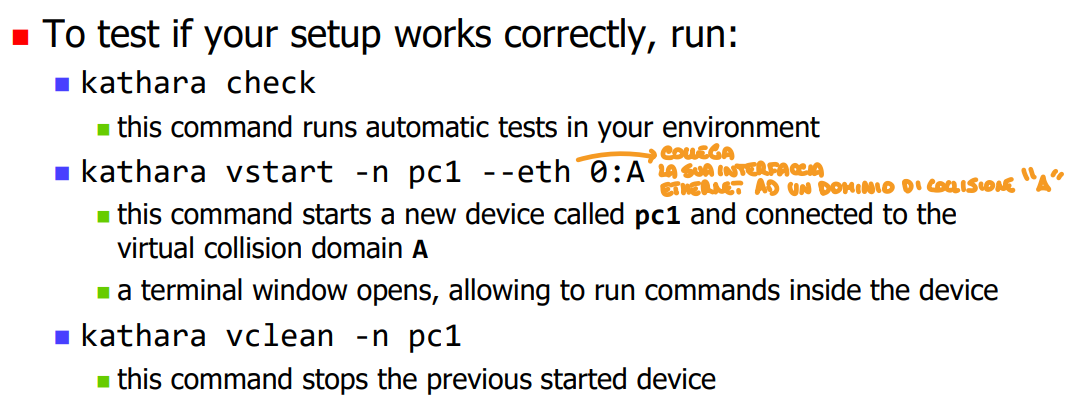
\includegraphics[width=13cm, height=5cm]{immagine_2024-12-26_172417199.png} % Percorso dell'immagine
    \caption{} % Didascalia per l'immagine
    \label{fig:immagine} % Etichetta per riferimento
\end{figure}
\noindent
In un lab Katharà solitamente c'è un \textbf{lab.conf} che descrive la topologia di rete e i dispositivi che vengono avviati, una serie di \textbf{sottocartelle} dove solitamente sono situate le impostazioni di configurazione per ogni dispositivo e i file \textbf{.startup} nei quali vengono scritte le azioni che esegue un dispositivo quando viene avviato.
\begin{figure}[H] % Usa 'H' per forzare la posizione qui
    \centering % Centra l'immagine
    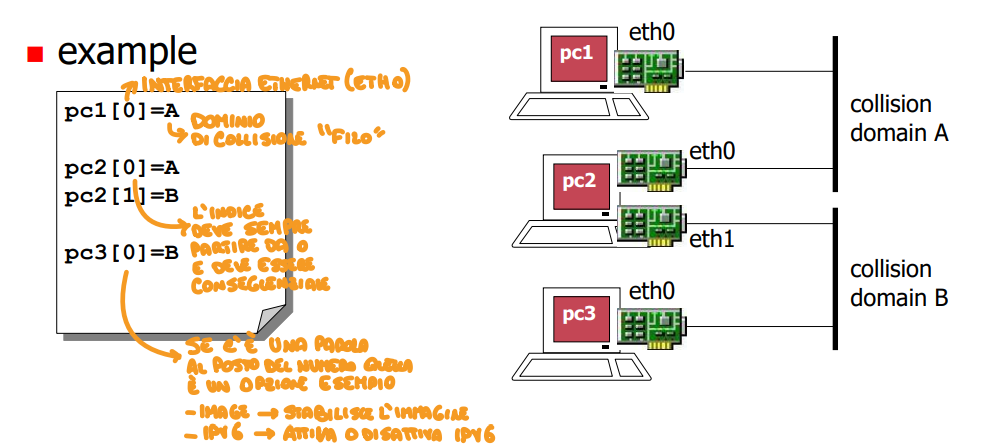
\includegraphics[width=13cm, height=5cm]{immagine_2024-12-26_172828613.png} % Percorso dell'immagine
    \caption{} % Didascalia per l'immagine
    \label{fig:immagine} % Etichetta per riferimento
\end{figure}
\noindent
\section{Primo Lab: due computer}
\begin{figure}[H] % Usa 'H' per forzare la posizione qui
    \centering % Centra l'immagine
    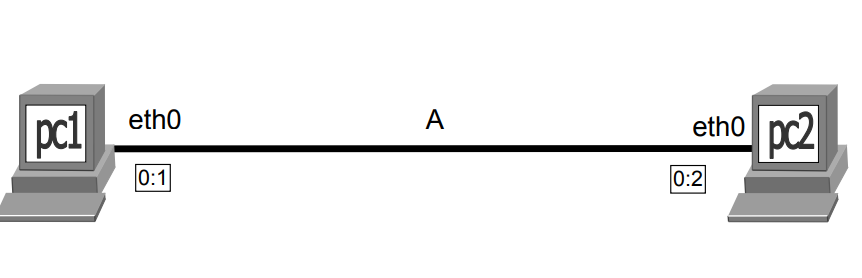
\includegraphics[width=13cm, height=3cm]{immagine_2025-01-02_125521028.png} % Percorso dell'immagine
    \caption{} % Didascalia per l'immagine
    \label{fig:immagine} % Etichetta per riferimento
\end{figure}
\noindent
Nel lab.conf notiamo come pc1 ha un'interfaccia (eth0) connessa a un dominio di collisione A. In questo lab l'indirizzo MAC è specificato, se non lo fosse, Katharà gliene assegnerebbe uno \textbf{random}. Per cambiare un indirizzo MAC:
\begin{figure}[H] % Usa 'H' per forzare la posizione qui
    \centering % Centra l'immagine
    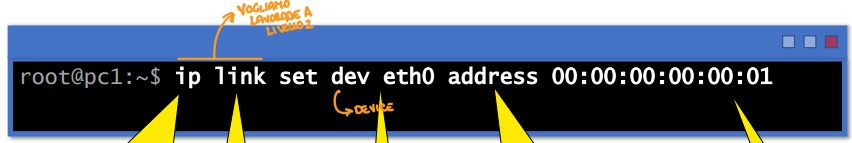
\includegraphics[width=13cm, height=2cm]{immagine_2024-12-26_173420516.png} % Percorso dell'immagine
    \caption{} % Didascalia per l'immagine
    \label{fig:immagine} % Etichetta per riferimento
\end{figure}
\noindent
Vogliamo far comunicare i due computer e lo facciamo con frame Ethernet (Frame di livello 2) a tal proposito utilizziamo scapy, basta digitare scapy nel dispositivo, mentre per uscirci exit(). Creiamo il pacchetto:
\begin{figure}[H] % Usa 'H' per forzare la posizione qui
    \centering % Centra l'immagine
    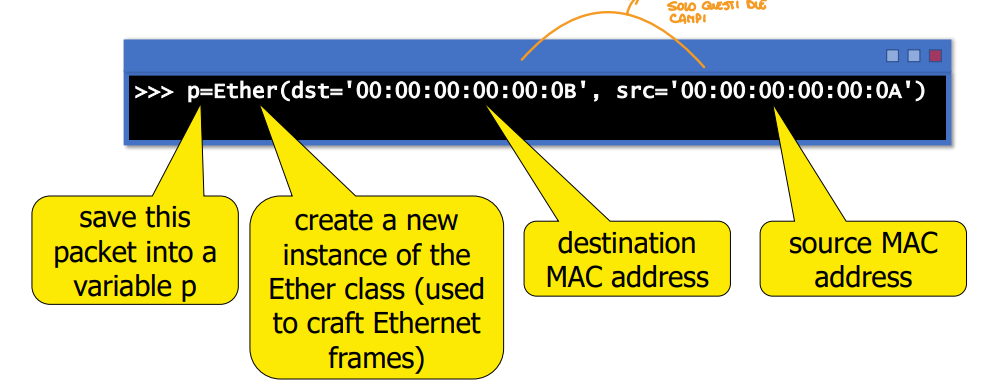
\includegraphics[width=13cm, height=5cm]{immagine_2024-12-26_173740029.png} % Percorso dell'immagine
    \caption{} % Didascalia per l'immagine
    \label{fig:immagine} % Etichetta per riferimento
\end{figure}
\noindent
Inviamo il pacchetto:
\begin{figure}[H] % Usa 'H' per forzare la posizione qui
    \centering % Centra l'immagine
    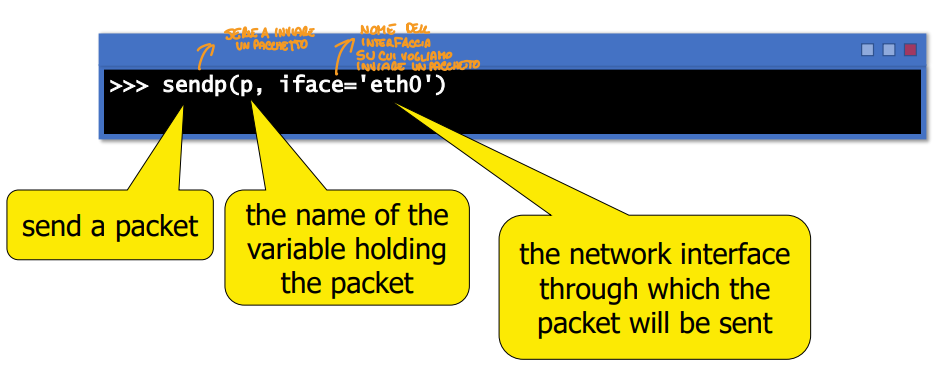
\includegraphics[width=13cm, height=5cm]{Screenshot 2024-12-26 173909.png} % Percorso dell'immagine
    \caption{} % Didascalia per l'immagine
    \label{fig:immagine} % Etichetta per riferimento
\end{figure}
\noindent
Per sapere se il pacchetto è stato ricevuto utilizziamo un \textbf{packet sniffer}, è uno strumento che cattura il traffico di rete che transita su un segmento di rete. A tal proposito utilizziamo \textbf{wireshark}. Per aprirlo basta digitare sulla barra di ricerca del browser \textbf{http://localhost:3000}. Ovviamente per analizzare il dominio di collisione bisogna \textbf{connettere} la macchina wireshark:
\begin{figure}[H] % Usa 'H' per forzare la posizione qui
    \centering % Centra l'immagine
    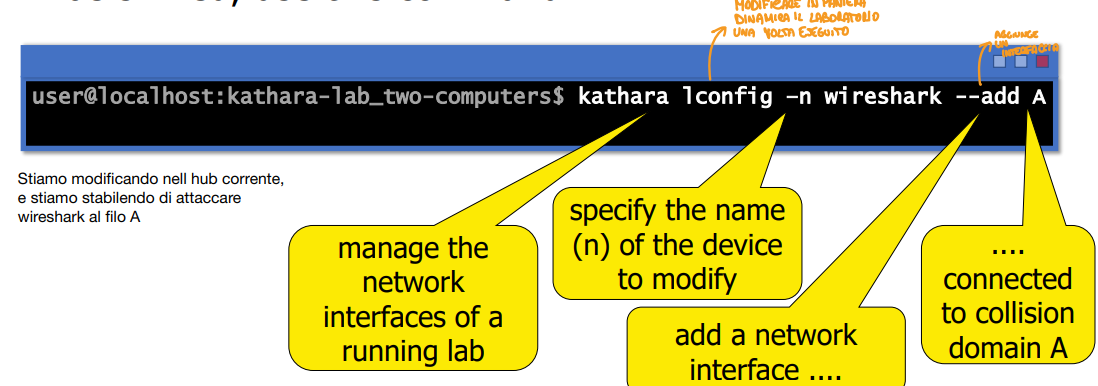
\includegraphics[width=14cm, height=5cm]{immagine_2024-12-26_174344833.png} % Percorso dell'immagine
    \caption{} % Didascalia per l'immagine
    \label{fig:immagine} % Etichetta per riferimento
\end{figure}
\noindent
\textbf{NOTA:} quando connettiamo wireshark a un dominio di collisione per essere sniffato, viene aggiunta un interfaccia. La dovremo aprire per analizzare il traffico di rete.
\section{Secondo Lab: un bridge}
\begin{figure}[H] % Usa 'H' per forzare la posizione qui
    \centering % Centra l'immagine
    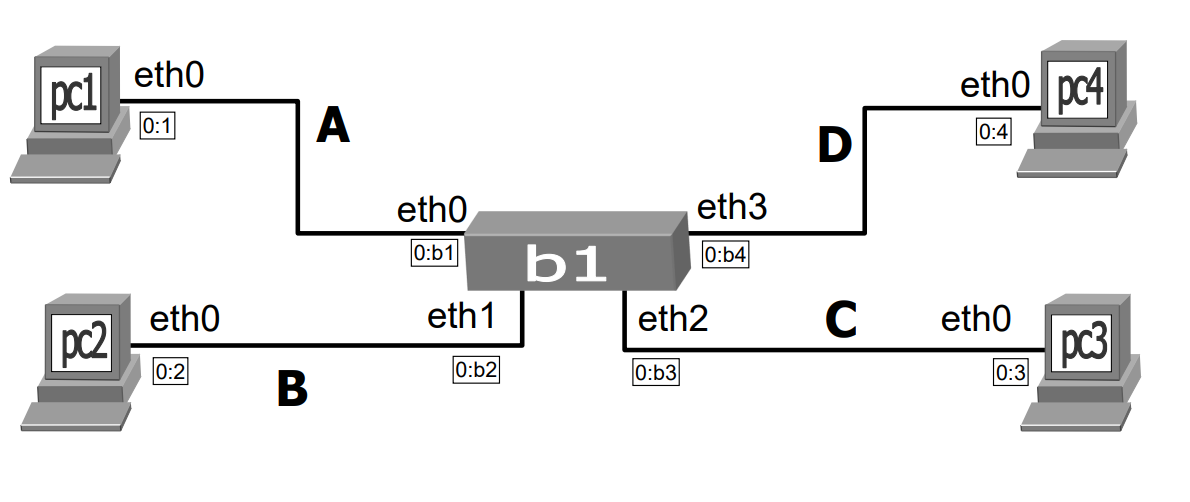
\includegraphics[width=14cm, height=4cm]{immagine_2025-01-02_125753713.png} % Percorso dell'immagine
    \caption{} % Didascalia per l'immagine
    \label{fig:immagine} % Etichetta per riferimento
\end{figure}
\noindent
Per prima cosa creiamo un bridge:
\begin{figure}[H] % Usa 'H' per forzare la posizione qui
    \centering % Centra l'immagine
    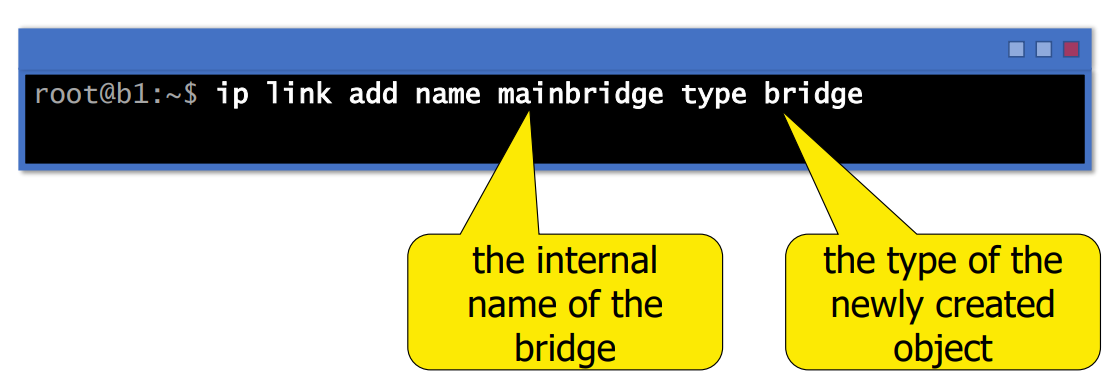
\includegraphics[width=14cm, height=4cm]{immagine_2024-12-27_113240386.png} % Percorso dell'immagine
    \caption{} % Didascalia per l'immagine
    \label{fig:immagine} % Etichetta per riferimento
\end{figure}
\noindent
Quindi andiamo a creare un oggetto bridge all'interno di b1. Successivamente connettiamo l'interfaccia eth0:
\begin{figure}[H] % Usa 'H' per forzare la posizione qui
    \centering % Centra l'immagine
    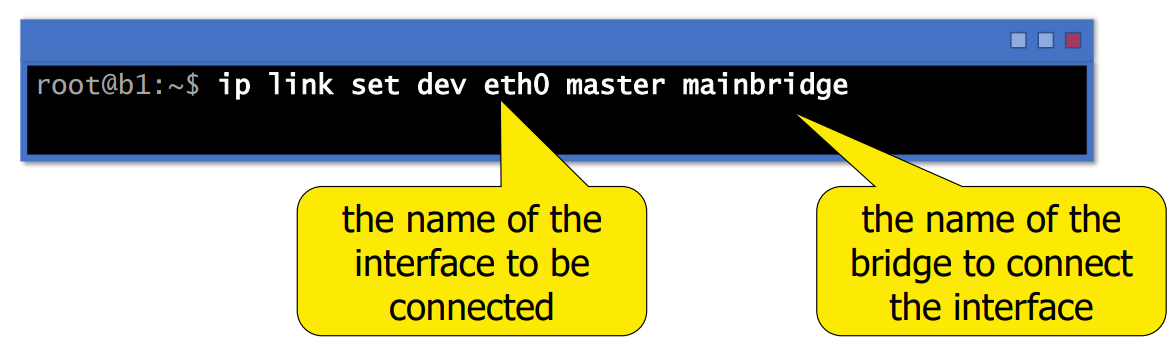
\includegraphics[width=14cm, height=4cm]{immagine_2024-12-27_113523358.png} % Percorso dell'immagine
    \caption{} % Didascalia per l'immagine
    \label{fig:immagine} % Etichetta per riferimento
\end{figure}
\noindent
Quando un bridge viene creato il suo stato iniziale è DOWN. Andiamo quindi a settare il suo stato su up:
\begin{figure}[H] % Usa 'H' per forzare la posizione qui
    \centering % Centra l'immagine
    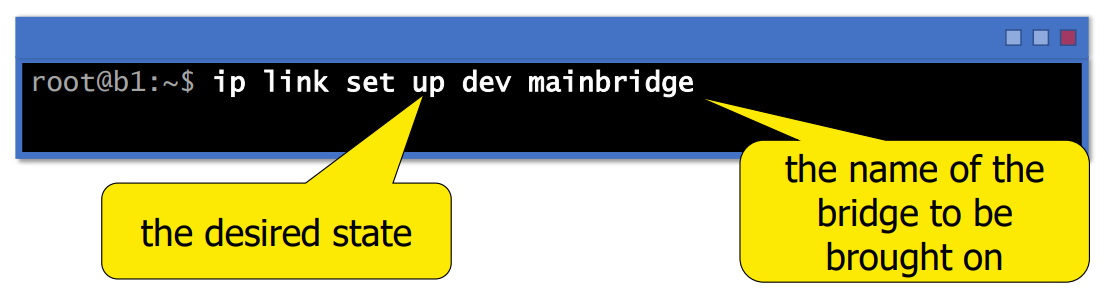
\includegraphics[width=15cm, height=4cm]{immagine_2024-12-27_113646349.png} % Percorso dell'immagine
    \caption{} % Didascalia per l'immagine
    \label{fig:immagine} % Etichetta per riferimento
\end{figure}
\noindent
I dati del filtering database non rimangono per sempre, di default dopo 300 s vengono tolti dal filtering database, possiamo cambiare il tempo ("ageing time") cosi:
\begin{figure}[H] % Usa 'H' per forzare la posizione qui
    \centering % Centra l'immagine
    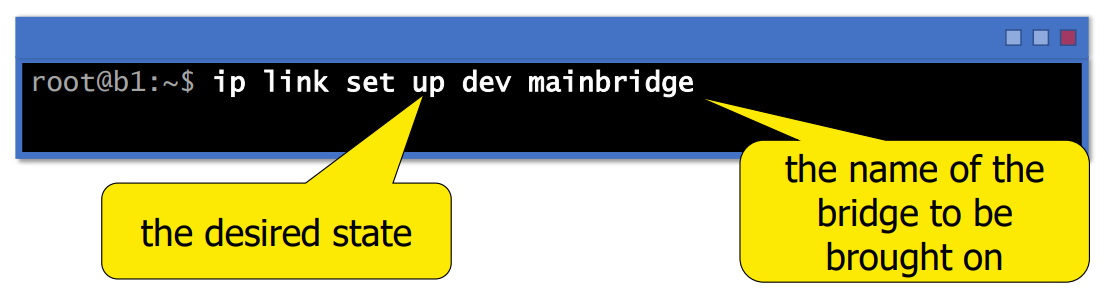
\includegraphics[width=15cm, height=4cm]{immagine_2024-12-27_113646349.png} % Percorso dell'immagine
    \caption{} % Didascalia per l'immagine
    \label{fig:immagine} % Etichetta per riferimento
\end{figure}
\noindent
Tutti questi comandi sono già presenti sul file di startup di b1. Andiamo ora ad analizzare il filtering database del bridge:
\begin{figure}[H] % Usa 'H' per forzare la posizione qui
    \centering % Centra l'immagine
    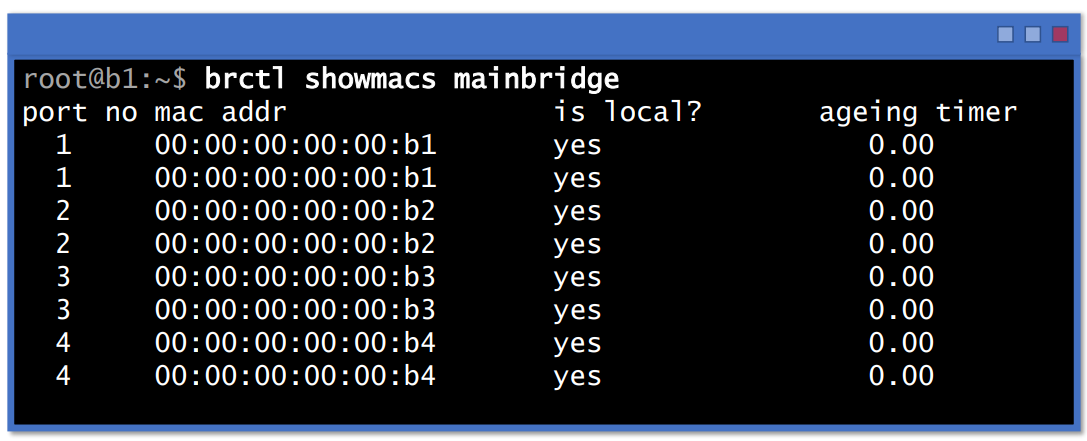
\includegraphics[width=15cm, height=6cm]{immagine_2024-12-27_114127744.png} % Percorso dell'immagine
    \caption{} % Didascalia per l'immagine
    \label{fig:immagine} % Etichetta per riferimento
\end{figure}
\noindent
Il bridge di Linux impara automaticamente i MAC address delle sue interfacce locali. L'ageing time è a 0 dato che le interfacce locali non scadono mai. Port indica il numero di porte virtuali del bridge. L'ageing time indica quanto questo indirizzo è rimasto nel filtering database. \\
Successivamente inviamo un pacchetto con scapy e ci accorgiamo che il filtering database impara il MAC addr del mittente.
\section{Terzo Lab: Configurazione di base IPv4, Ping, Traceroute e Arp}
\begin{figure}[H] % Usa 'H' per forzare la posizione qui
    \centering % Centra l'immagine
    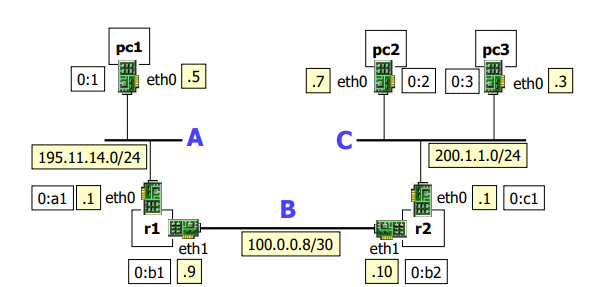
\includegraphics[width=12cm, height=5cm]{immagine_2025-01-02_130342499.png} % Percorso dell'immagine
    \caption{} % Didascalia per l'immagine
    \label{fig:immagine} % Etichetta per riferimento
\end{figure}
\noindent
Nel lab.conf assegnamo a ogni host, un indirizzo IPv4 alle loro interfacce eth0. Inoltre aggiungiamo per ogni host, un default gateway.
\begin{figure}[H] % Usa 'H' per forzare la posizione qui
    \centering % Centra l'immagine
    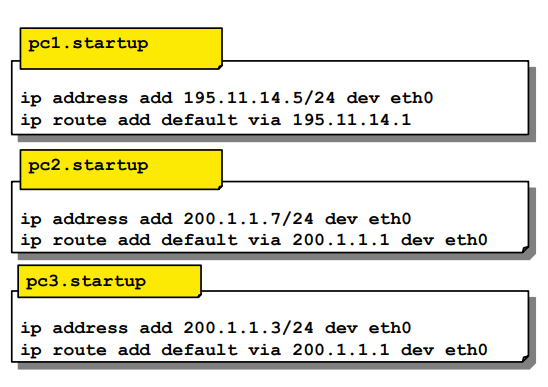
\includegraphics[width=10cm, height=6cm]{immagine_2024-12-30_143439466.png} % Percorso dell'immagine
    \caption{} % Didascalia per l'immagine
    \label{fig:immagine} % Etichetta per riferimento
\end{figure}
\noindent
Configuriamo anche i router, a cui aggiungiamo i collegamenti alle macchine e il next hop.
\begin{figure}[H] % Usa 'H' per forzare la posizione qui
    \centering % Centra l'immagine
    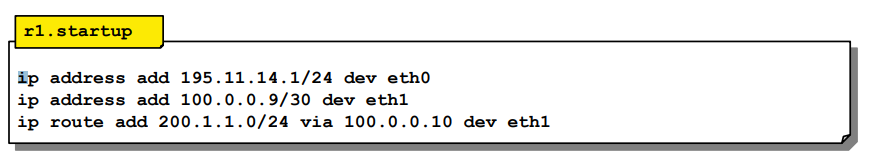
\includegraphics[width=10cm, height=2cm]{immagine_2024-12-30_143729333.png} % Percorso dell'immagine
    \caption{} % Didascalia per l'immagine
    \label{fig:immagine} % Etichetta per riferimento
\end{figure}
\noindent
Per vedere gli indirizzi assegnati alle interfacce eseguiamo il comando: ip address.
\begin{figure}[H] % Usa 'H' per forzare la posizione qui
    \centering % Centra l'immagine
    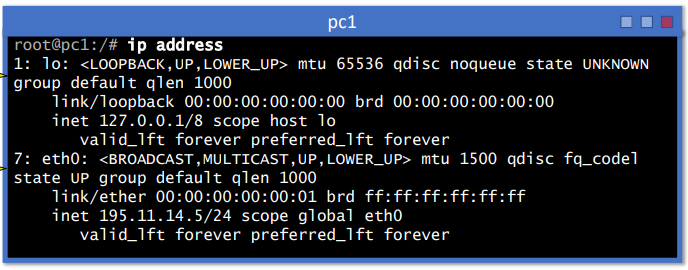
\includegraphics[width=12cm, height=5cm]{immagine_2024-12-30_143940102.png} % Percorso dell'immagine
    \caption{} % Didascalia per l'immagine
    \label{fig:immagine} % Etichetta per riferimento
\end{figure}
\noindent
Per vedere se è presente una rotta di default utilizziamo routel
\begin{figure}[H] % Usa 'H' per forzare la posizione qui
    \centering % Centra l'immagine
    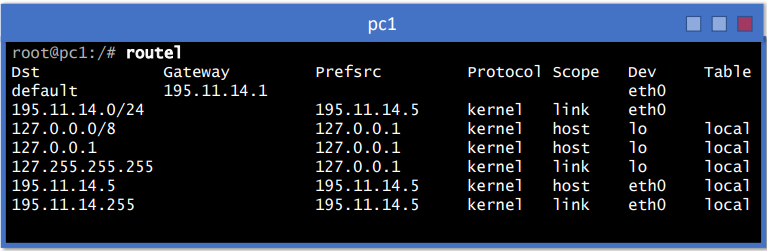
\includegraphics[width=14cm, height=5cm]{Screenshot 2024-12-30 144305.png} % Percorso dell'immagine
    \caption{} % Didascalia per l'immagine
    \label{fig:immagine} % Etichetta per riferimento
\end{figure}
\noindent
Se lo utilizziamo invece sul router possiamo vedere la tabella di instradamento. Ora vogliamo vedere il comportamento ARP. In particolare andiamo a vedere prima la tabella ARP senza l'invio di nessun pacchetto:
\begin{figure}[H] % Usa 'H' per forzare la posizione qui
    \centering % Centra l'immagine
    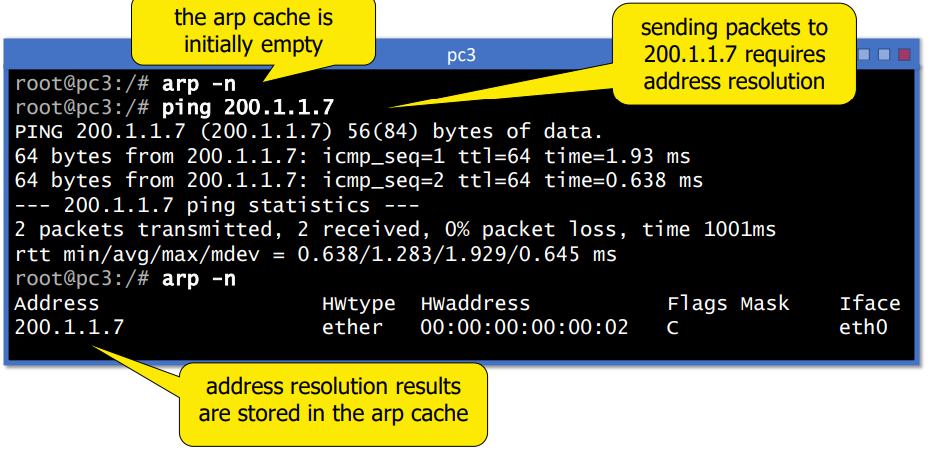
\includegraphics[width=14cm, height=5cm]{immagine_2024-12-30_145009848.png} % Percorso dell'immagine
    \caption{} % Didascalia per l'immagine
    \label{fig:immagine} % Etichetta per riferimento
\end{figure}
\noindent
Inizialmente il comando non restituirà nulla essendo essendo l'ARP cache vuota, dopo aver eseguito da pc3 un ping a pc2 memorizzerà, l'indirizzo di pc2. Le comunicazioni sono \textbf{bidirezionali}, infatti una volta aver ricevuto un \textbf{ARP Request} anche il destinatario memorizzerà nell \textbf{ARP cache} l'indirizzo del mittente. Con Wireshark possiamo osservare i pacchetti ARP, in particolare \textbf{ARP Request} e \textbf{ARP Reply}. Notiamo successivamente che alla fine del ping vi è un ulteriore arp request/reply unicast. \\
Ora ripetiamo lo stesso esperimento su due computer che stavolta, non sono sulla stessa LAN. Questa volta su pc2 verrà memorizzato l'indirizzo del primo Router (r2) che inoltra la sua richiesta. Quando arriva una ARP request a un Router loro la eseguono a loro volta, memorizzandone \textbf{mittente} e \textbf{destinatario/altro router} (se dovesse raggiungere un'altro router rifarà la stessa cosa).
\begin{figure}[H] % Usa 'H' per forzare la posizione qui
    \centering % Centra l'immagine
    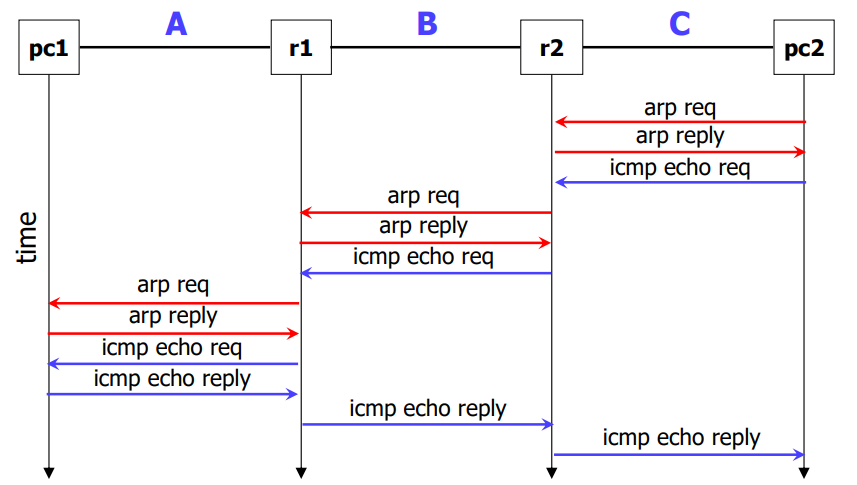
\includegraphics[width=14cm, height=5cm]{Screenshot 2024-12-30 150054.png} % Percorso dell'immagine
    \caption{} % Didascalia per l'immagine
    \label{fig:immagine} % Etichetta per riferimento
\end{figure}
\noindent
Andiamo ora ad analizzare \textbf{Traceroute}
\begin{figure}[H] % Usa 'H' per forzare la posizione qui
    \centering % Centra l'immagine
    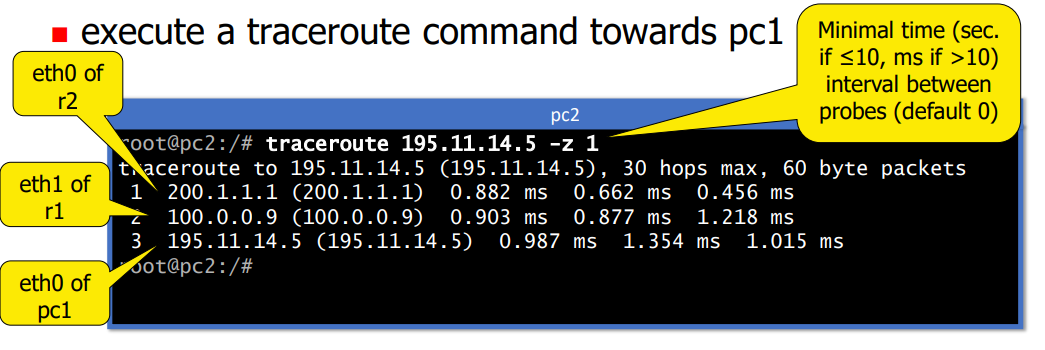
\includegraphics[width=14cm, height=5cm]{Screenshot 2024-12-30 150333.png} % Percorso dell'immagine
    \caption{} % Didascalia per l'immagine
    \label{fig:immagine} % Etichetta per riferimento
\end{figure}
\noindent
Analizzando wireshark osserviamo i pacchetti con \textbf{TTL} basso e i relativi \textbf{Time-to-live exceeded} da parte di ICMP. Cliccando sul pacchetto è possibile vedere il TTL del pacchetto in basso a sinistra. In questo caso venivano mandati 3 pacchetti e poi veniva incrementato il \textbf{TTL}. Durante il dialogo avvengono degli arp unicast query.
\section{Quarto Lab: IPv6 Configurazione di base, ping, traceroute e ICMPv6}
\begin{figure}[H] % Usa 'H' per forzare la posizione qui
    \centering % Centra l'immagine
    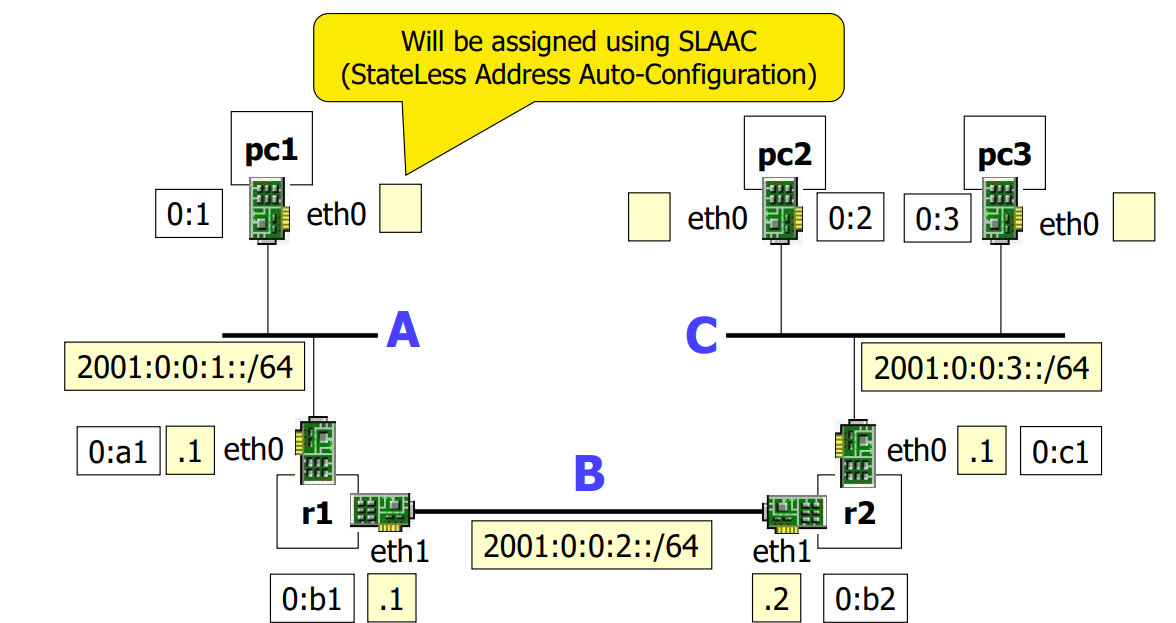
\includegraphics[width=12cm, height=5cm]{immagine_2025-01-02_130441787.png} % Percorso dell'immagine
    \caption{} % Didascalia per l'immagine
    \label{fig:immagine} % Etichetta per riferimento
\end{figure}
\noindent
Le differenze rispetto ai lab visti fino ad ora sono poche, in particolare utilizziamo gli indirizzi IPv6 e a ogni pc inseriamo il comando che accetta i router advertisement. Sullo startup non c'è nulla dato che c'è l'\textbf{autoconfigurazione stateless}.
\begin{figure}[H] % Usa 'H' per forzare la posizione qui
    \centering % Centra l'immagine
    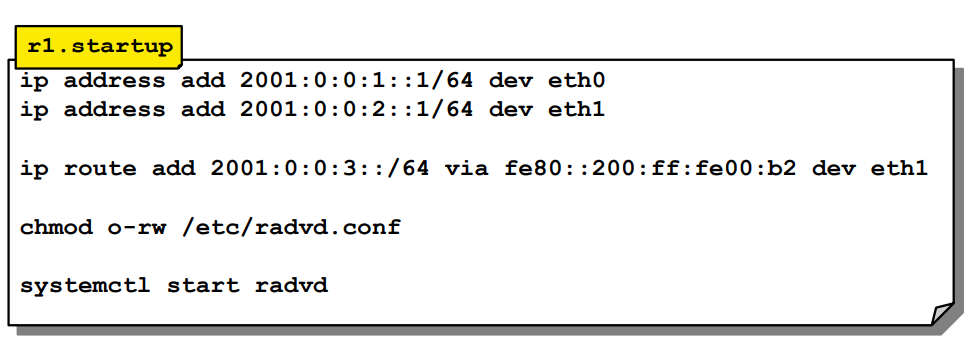
\includegraphics[width=12cm, height=4cm]{immagine_2025-01-02_131006246.png} % Percorso dell'immagine
    \caption{} % Didascalia per l'immagine
    \label{fig:immagine} % Etichetta per riferimento
\end{figure}
\noindent
Vengono messi degli indirizzi IPv6 alle interfacce del router. Viene inoltre aggiunta una riga per far capire al router come raggiungere una LAN che non è direttamente connessa. Il nexthop è un indirizzo link-local. La linea in cui c'è chmod serve a mettere i privilegi corretti per radvd.conf e inizializzare il servizio radvd (router advertisement). Il suo configuration file è nella cartella di r1.
\begin{figure}[H] % Usa 'H' per forzare la posizione qui
    \centering % Centra l'immagine
    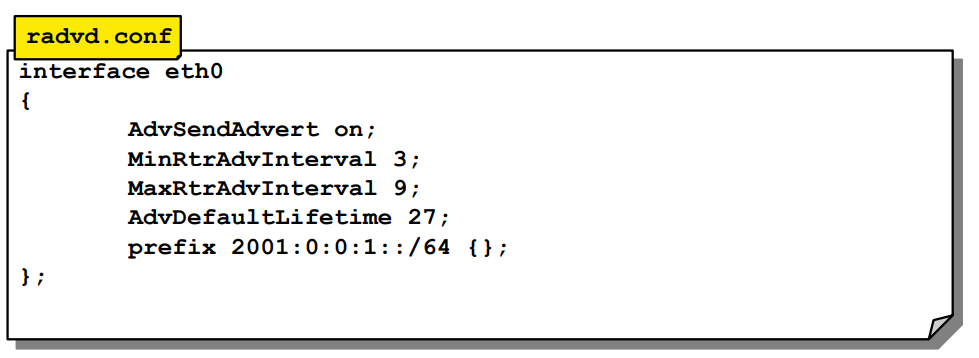
\includegraphics[width=12cm, height=4cm]{immagine_2025-01-02_134051773.png} % Percorso dell'immagine
    \caption{} % Didascalia per l'immagine
    \label{fig:immagine} % Etichetta per riferimento
\end{figure}
\noindent
In questo file andiamo a specificare dove il router manderà gli advertisement (interface eth0), andiamo a mettere in on il fatto che il router manderà gli advertisement, settiamo il massimo e minimo intervallo tra advertisement consecutivi, il tempo di intervallo di default per la validità del gateway e il prefisso annunciato. Come per IPv4 utilizziamo \textbf{ip address} per vedere le interfacce IPv6 di r1.
\begin{figure}[H] % Usa 'H' per forzare la posizione qui
    \centering % Centra l'immagine
    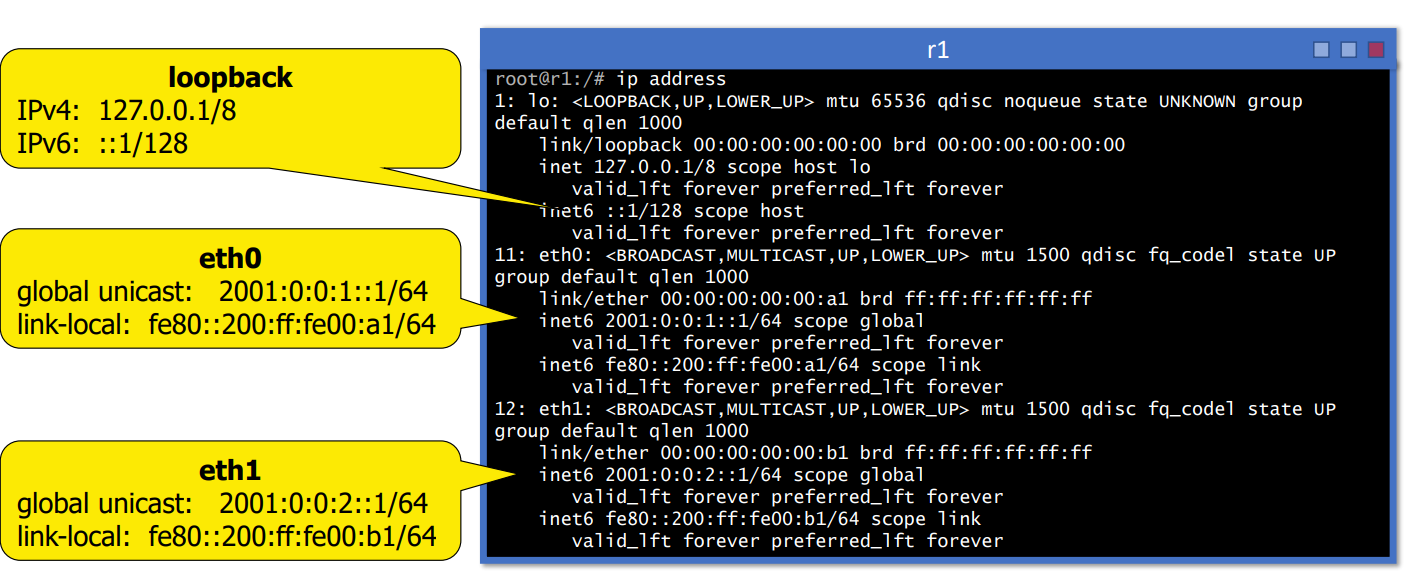
\includegraphics[width=16cm, height=7cm]{immagine_2025-01-02_134616748.png} % Percorso dell'immagine
    \caption{} % Didascalia per l'immagine
    \label{fig:immagine} % Etichetta per riferimento
\end{figure}
\noindent
Questa volta per vedere la tabella di instradamento IPv6 utilizziamo \textbf{routel -6}. Utilizziamo \textbf{ip address} sulle macchine per vedere l'indirizzo IPv6 assegnato automaticamente. Utilizziamo \textbf{routel -6} per controllare la presenza di una rotta di default. Ora attacchiamo wireshark per vedere il comportamento di \textbf{ICMPv6}. Quindi su \textbf{pc3} ispezioniamo la neighbor cache (ARP cache di IPv6) facciamo un ping a \textbf{pc2}, ricontrolliamo la cache e osserviamo i pacchetti che ha catturato wireshark. Quello che notiamo è che ora \textbf{pc3} ha nella neighbor cache l'indirizzo globale IPv6 di \textbf{pc2}. Anche qui le comunicazioni sono bidirezionali di conseguenza anche \textbf{pc2} avrà memorizzato l'indirizzo globale IPv6 di \textbf{pc3}.
\begin{figure}[H] % Usa 'H' per forzare la posizione qui
    \centering % Centra l'immagine
    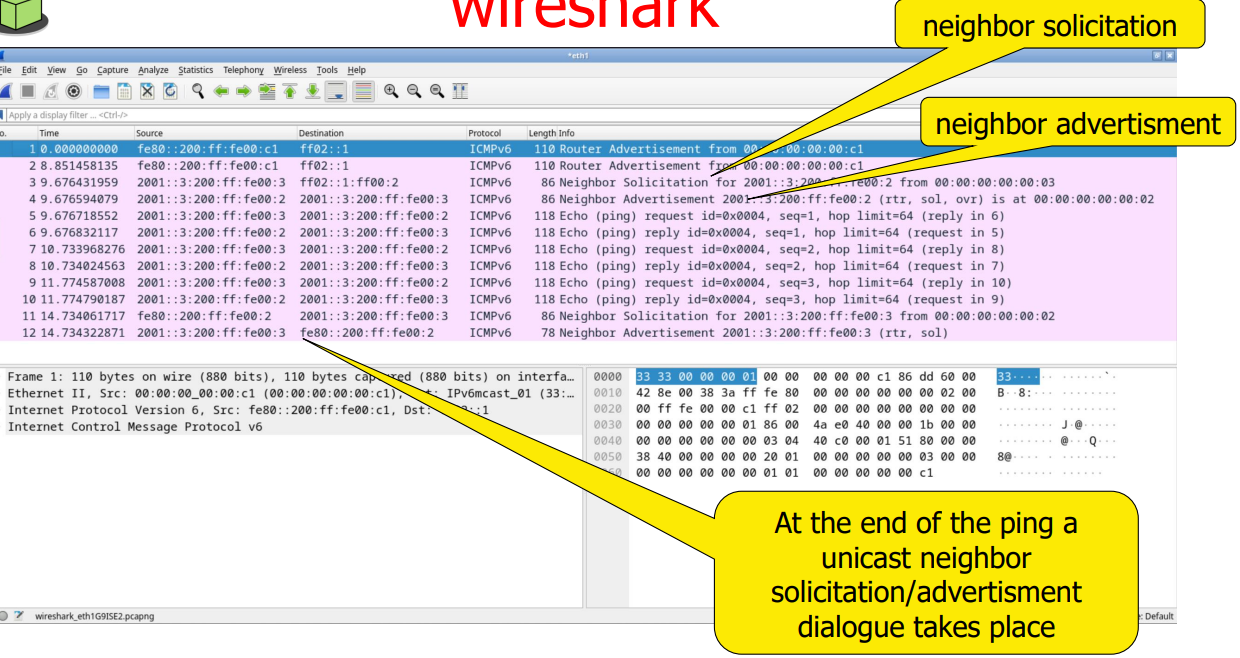
\includegraphics[width=16cm, height=9cm]{immagine_2025-01-02_135539978.png} % Percorso dell'immagine
    \caption{} % Didascalia per l'immagine
    \label{fig:immagine} % Etichetta per riferimento
\end{figure}
\noindent
Ora dopo aver aggiunto wireshark al dominio di collisione B vogliamo osservare cosa succede facendo un ping da pc2 a pc1. pc2 impara il mac address di r2 su eth0. 
\begin{figure}[H] % Usa 'H' per forzare la posizione qui
    \centering % Centra l'immagine
    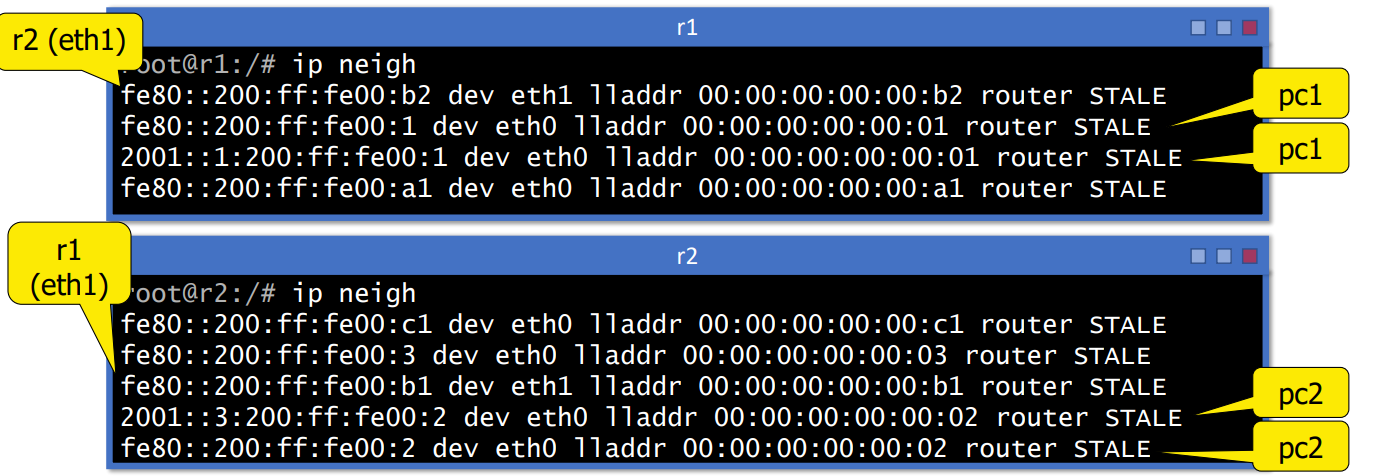
\includegraphics[width=16cm, height=4cm]{Screenshot 2025-01-02 135934.png} % Percorso dell'immagine
    \caption{} % Didascalia per l'immagine
    \label{fig:immagine} % Etichetta per riferimento
\end{figure}
\noindent
Su wireshark osserviamo un Neighbor Solicitation per capire quale fosse il mac address di r1.
\begin{figure}[H] % Usa 'H' per forzare la posizione qui
    \centering % Centra l'immagine
    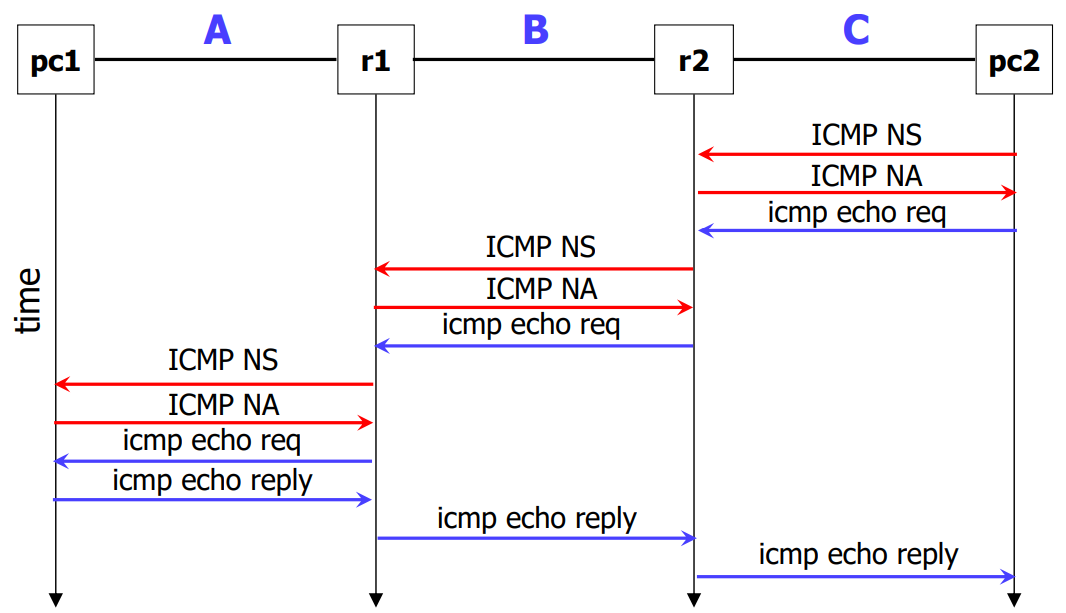
\includegraphics[width=13cm, height=5cm]{immagine_2025-01-02_140314841.png} % Percorso dell'immagine
    \caption{} % Didascalia per l'immagine
    \label{fig:immagine} % Etichetta per riferimento
\end{figure}
\noindent
Ora vogliamo osservare il comportamento di ICMPv6 facendo traceroute da pc2 a pc1, per farlo attacchiamo wireshark al dominio di collisione C.
\begin{figure}[H] % Usa 'H' per forzare la posizione qui
    \centering % Centra l'immagine
    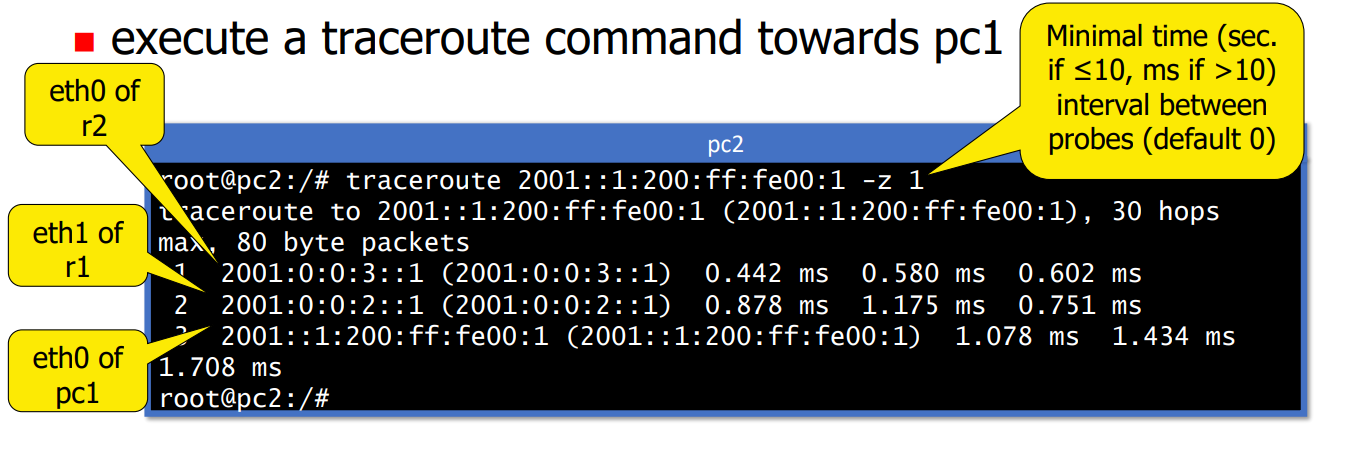
\includegraphics[width=15cm, height=6cm]{Screenshot 2025-01-02 140502.png} % Percorso dell'immagine
    \caption{} % Didascalia per l'immagine
    \label{fig:immagine} % Etichetta per riferimento
\end{figure}
\noindent
Osserviamo quindi pacchetti \textbf{UDP} e pacchetti \textbf{ICMP Time-To-Live exceeded}
\section{Quinto Lab: DNS}
\begin{figure}[H] % Usa 'H' per forzare la posizione qui
    \centering % Centra l'immagine
    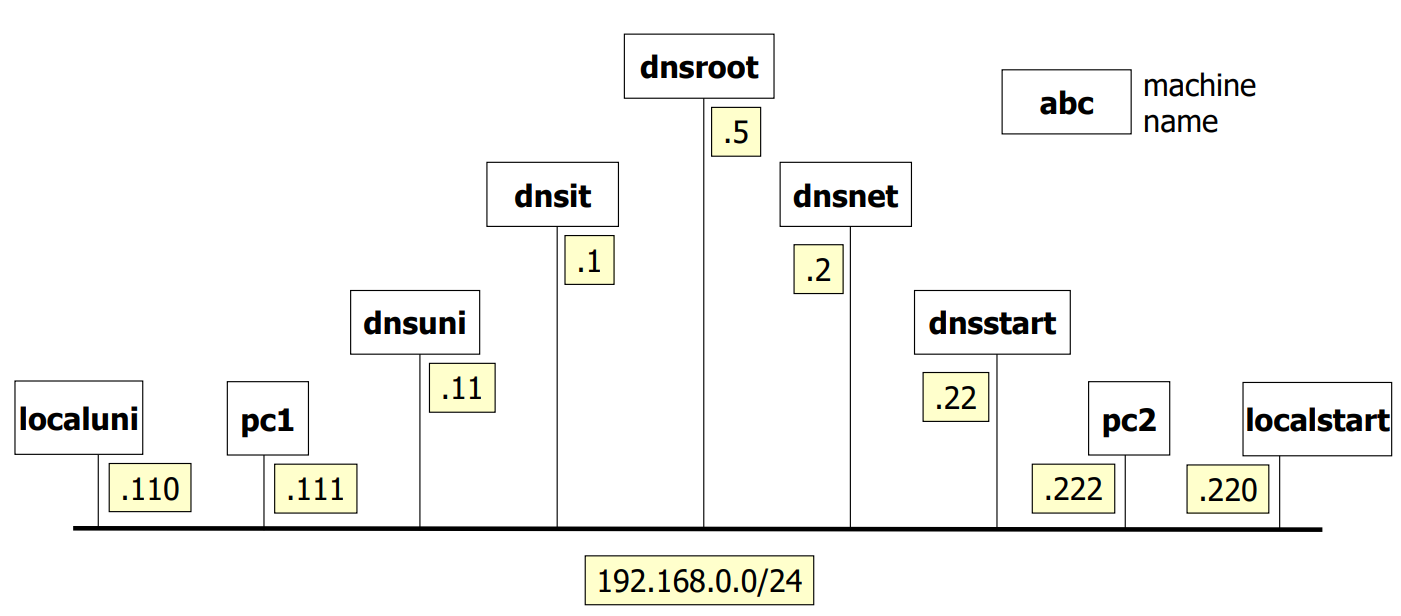
\includegraphics[width=15cm, height=5cm]{immagine_2025-01-04_115729575.png} % Percorso dell'immagine
    \caption{} % Didascalia per l'immagine
    \label{fig:immagine} % Etichetta per riferimento
\end{figure}
\noindent
\begin{figure}[H] % Usa 'H' per forzare la posizione qui
    \centering % Centra l'immagine
    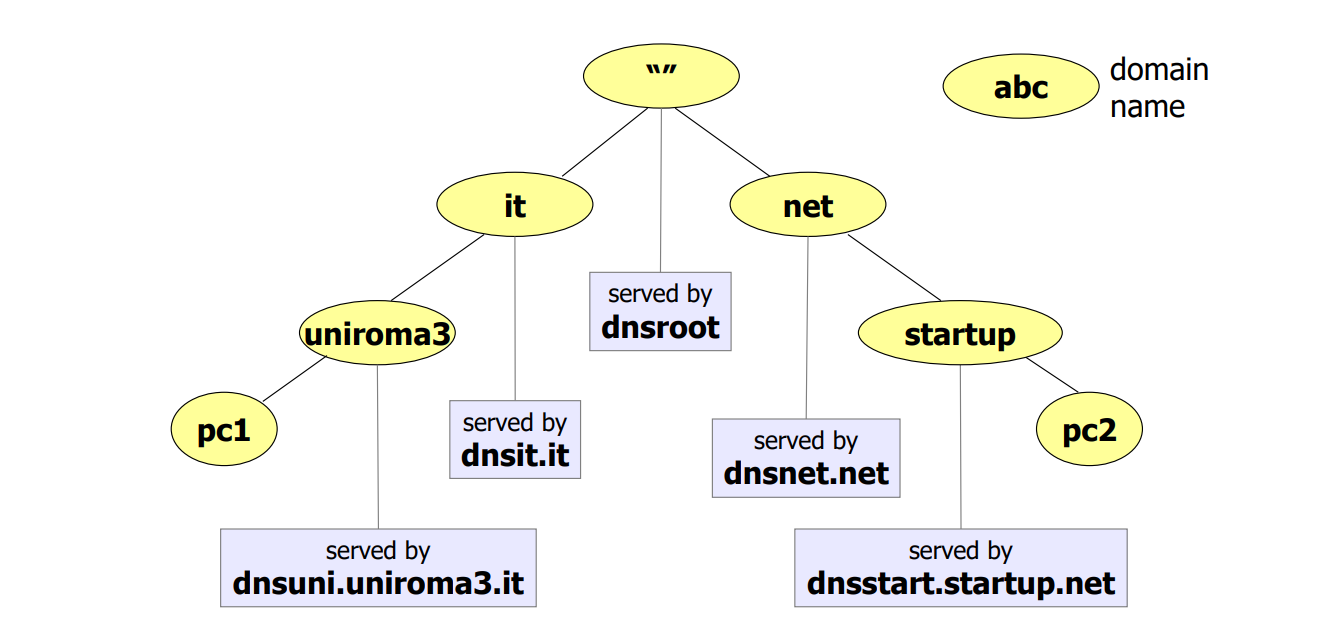
\includegraphics[width=15cm, height=4cm]{immagine_2025-01-04_115818891.png} % Percorso dell'immagine
    \caption{} % Didascalia per l'immagine
    \label{fig:immagine} % Etichetta per riferimento
\end{figure}
\noindent
La configurazione dei vari PC consiste sostanzialmente nello specificare il \textbf{default name server}
\begin{figure}[H] % Usa 'H' per forzare la posizione qui
    \centering % Centra l'immagine
    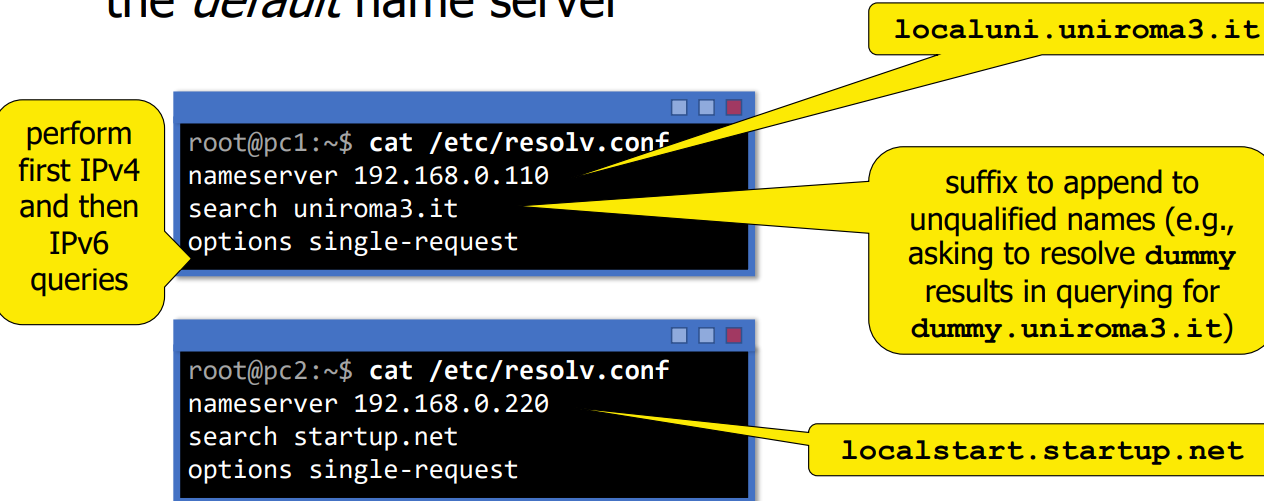
\includegraphics[width=15cm, height=4cm]{immagine_2025-01-04_120100344.png} % Percorso dell'immagine
    \caption{} % Didascalia per l'immagine
    \label{fig:immagine} % Etichetta per riferimento
\end{figure}
\noindent
Sui name server invece vengono specificati: associazioni tra zone e name server, informazioni sulla radice dei name server, associazioni tra nomi e indirizzi IP e l autorizzazione a risolvere query ricorsive.
\begin{figure}[H] % Usa 'H' per forzare la posizione qui
    \centering % Centra l'immagine
    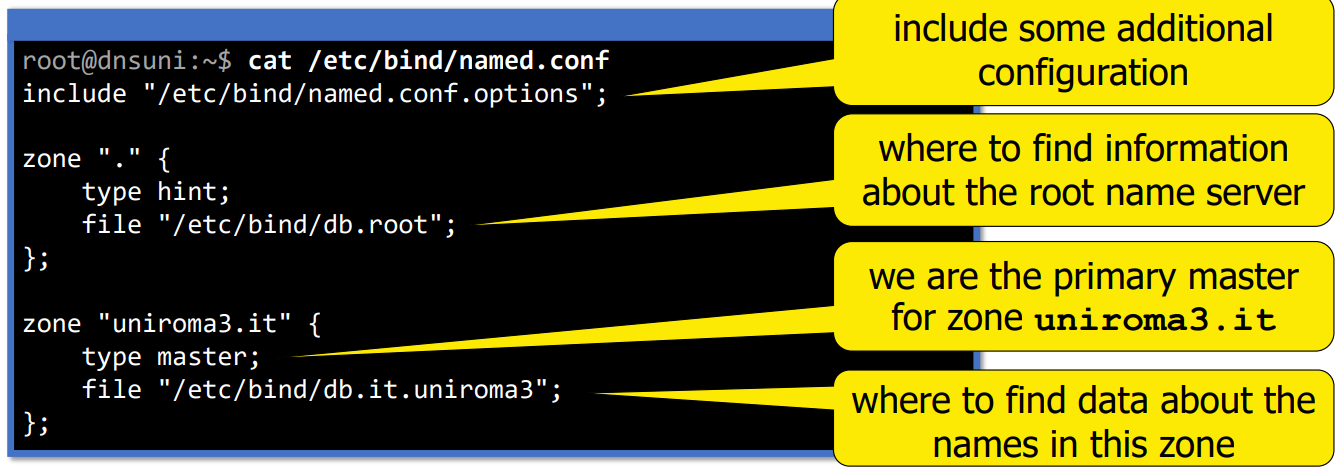
\includegraphics[width=15cm, height=5cm]{Screenshot 2025-01-04 120422.png} % Percorso dell'immagine
    \caption{} % Didascalia per l'immagine
    \label{fig:immagine} % Etichetta per riferimento
\end{figure}
\noindent
\begin{figure}[H] % Usa 'H' per forzare la posizione qui
    \centering % Centra l'immagine
    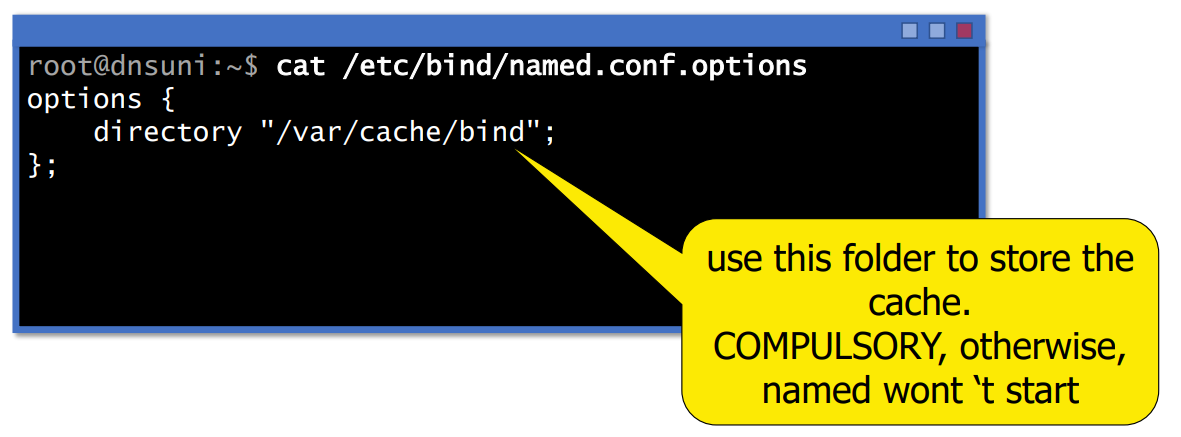
\includegraphics[width=15cm, height=5cm]{Screenshot 2025-01-04 120432.png} % Percorso dell'immagine
    \caption{} % Didascalia per l'immagine
    \label{fig:immagine} % Etichetta per riferimento
\end{figure}
\noindent
Informazioni sulla radice dei name server
\begin{figure}[H] % Usa 'H' per forzare la posizione qui
    \centering % Centra l'immagine
    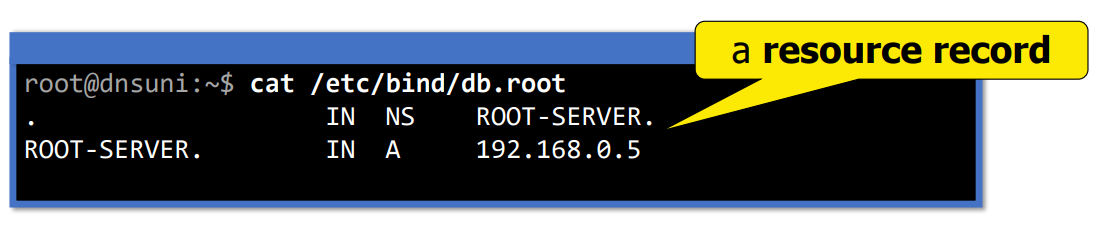
\includegraphics[width=15cm, height=3cm]{immagine_2025-01-04_120734535.png} % Percorso dell'immagine
    \caption{} % Didascalia per l'immagine
    \label{fig:immagine} % Etichetta per riferimento
\end{figure}
\noindent
Informazioni come il TTL e altre
\begin{figure}[H] % Usa 'H' per forzare la posizione qui
    \centering % Centra l'immagine
    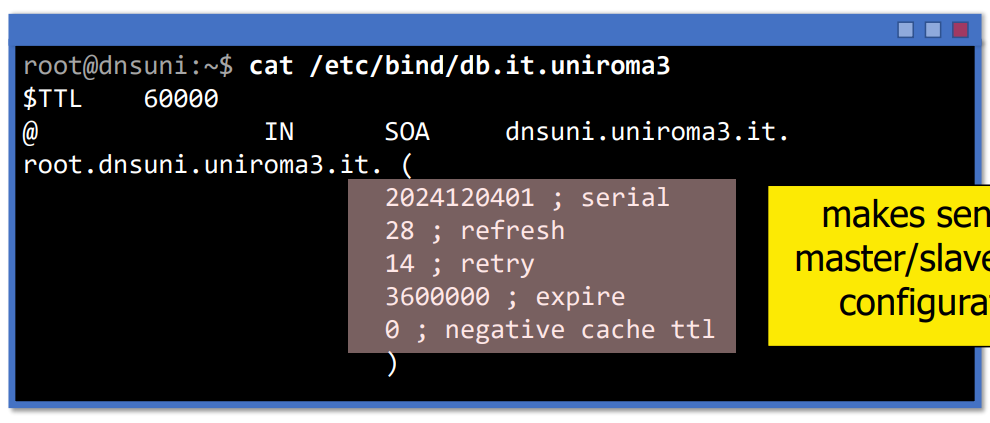
\includegraphics[width=15cm, height=5cm]{Screenshot 2025-01-04 121620.png} % Percorso dell'immagine
    \caption{} % Didascalia per l'immagine
    \label{fig:immagine} % Etichetta per riferimento
\end{figure}
\noindent
La chiocciola in alto a sinistra sta ad indicare che questo record si riferisce all'origine attuale, Tutti i nomi di dominio in questo file di dati che non sono completamente qualificati (non terminano con un ‘.’) sono relativi all'origine. L'\textbf{origine} è il nome di dominio nella dichiarazione della zona del file di configurazione del server. La riga che riporta \textbf{IN SOA dnsuni.uniroma3.it.} sta ad indicare il server master primario per questa zona (dnsuni.uniroma3.it), non bisogna dimenticare il punto finale altrimenti il nome dell'origine (uniroma3.it) verrebbe aggiunto. La riga che riporta \textbf{root.dnsuni.uniroma3.it} è l'indirizzo email della persona responsabile per quella zona (il primo . va scambiato con una @ root@dnsuni.uniroma3.it). Le righe evidenziate nella foto servono per le configurazioni dei server master e slave. \textbf{Serial number} indica quanto recente è l'informazione (è una data YYYYMMDDNN). \textbf{Refresh interval} indica allo slave quando spesso controllare i dati della zona se sono aggiornati. \textbf{Interval} è l'intervallo tra tentativi consecutivi per ricontattare il master. \textbf{Slave expire time} se lo slave fallisce a contattare il master per questa quantità di tempo, considera i dati della zona troppo vecchi e smette di dare informazioni su quest ultima. \textbf{TTL per responsi negativi}.
\begin{figure}[H] % Usa 'H' per forzare la posizione qui
    \centering % Centra l'immagine
    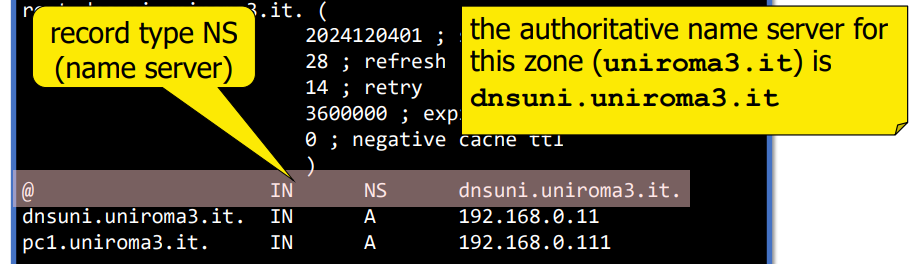
\includegraphics[width=15cm, height=5cm]{Screenshot 2025-01-04 124703.png} % Percorso dell'immagine
    \caption{} % Didascalia per l'immagine
    \label{fig:immagine} % Etichetta per riferimento
\end{figure}
\noindent
Sono segnate le macchine presenti in questa zona.
\begin{figure}[H] % Usa 'H' per forzare la posizione qui
    \centering % Centra l'immagine
    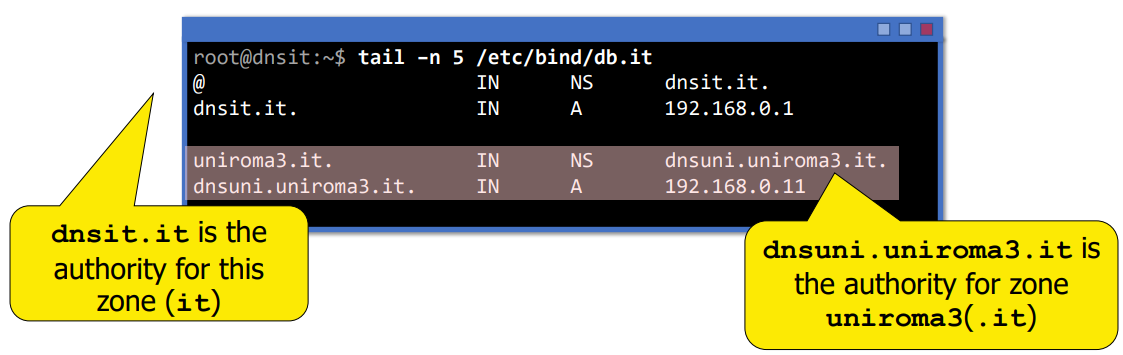
\includegraphics[width=15cm, height=5cm]{Screenshot 2025-01-04 124937.png} % Percorso dell'immagine
    \caption{} % Didascalia per l'immagine
    \label{fig:immagine} % Etichetta per riferimento
\end{figure}
\begin{figure}[H] % Usa 'H' per forzare la posizione qui
    \centering % Centra l'immagine
    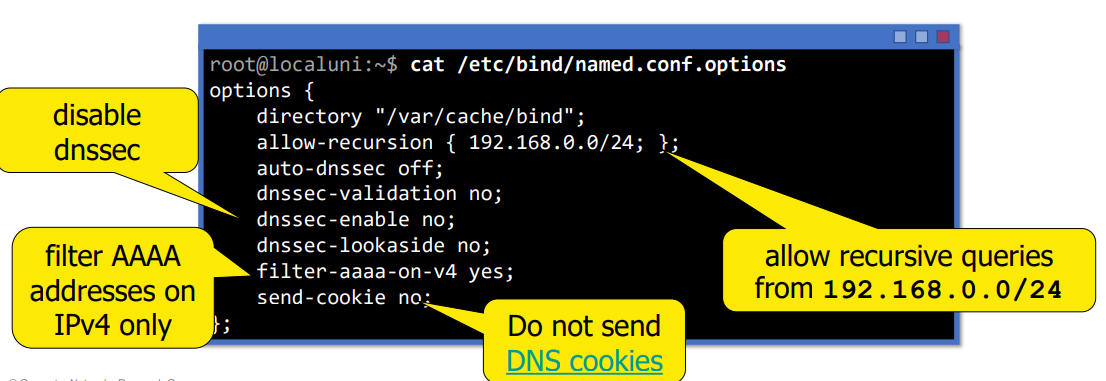
\includegraphics[width=15cm, height=5cm]{immagine_2025-01-04_125113037.png} % Percorso dell'immagine
    \caption{} % Didascalia per l'immagine
    \label{fig:immagine} % Etichetta per riferimento
\end{figure}
\noindent
Ora iniziamo il lab, aggiungiamo wireshark al dominio di collisione a e facciamo un ping da pc1 a pc2.
\begin{figure}[H] % Usa 'H' per forzare la posizione qui
    \centering % Centra l'immagine
    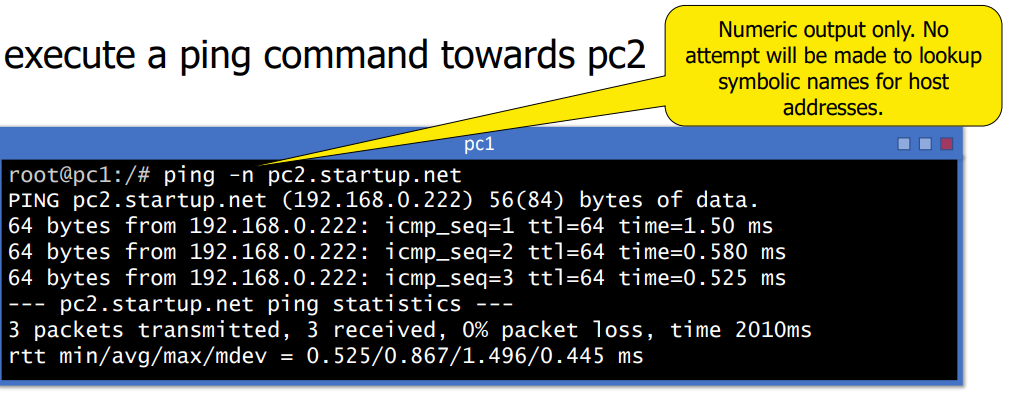
\includegraphics[width=15cm, height=5cm]{Screenshot 2025-01-04 125254.png} % Percorso dell'immagine
    \caption{} % Didascalia per l'immagine
    \label{fig:immagine} % Etichetta per riferimento
\end{figure}
\noindent
Applicando su wireshark il filtro per vedere sono i pacchetti DNS, possiamo notare tutte le varie query
\begin{figure}[H] % Usa 'H' per forzare la posizione qui
    \centering % Centra l'immagine
    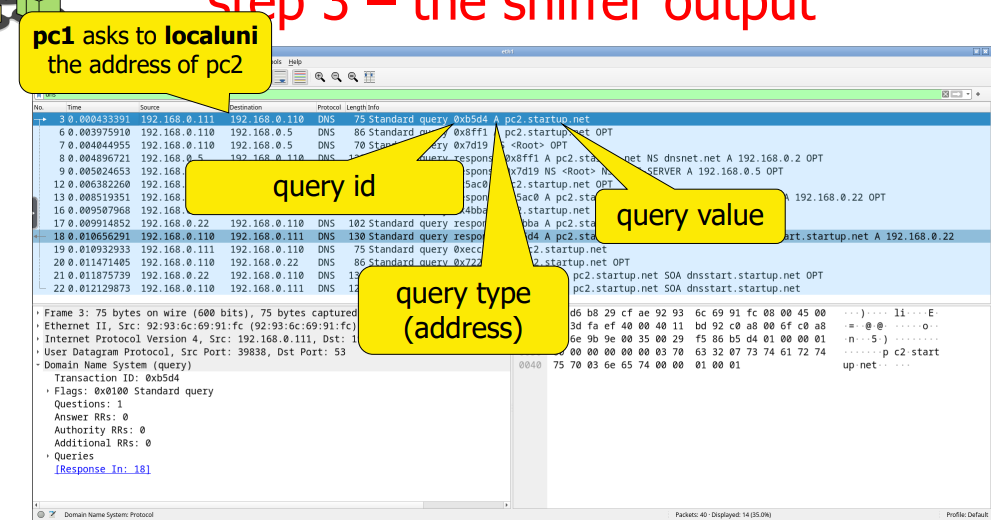
\includegraphics[width=16cm, height=9cm]{immagine_2025-01-04_125443044.png} % Percorso dell'immagine
    \caption{} % Didascalia per l'immagine
    \label{fig:immagine} % Etichetta per riferimento
\end{figure}
\noindent
Con \textbf{$<Root>$} possiamo vedere le richieste root name server. Quindi quello che succede è \textbf{pc1} chiede a \textbf{localuni} l'indirizzo di \textbf{pc2} il quale a sua volta chiede a \textbf{dnsroot} qual è il name server per il dominio net, riceve risposta \textbf{192.168.0.2}. Successivamente \textbf{localuni} chiede a \textbf{dnsnet} chi è il name server per il dominio \textbf{startup.net}. Riceve risposta, l'indirizzo di \textbf{dnsstart.startup.net} è \textbf{192.168.0.22.} Successivamente \textbf{localuni} chiede a \textbf{dnsstart} qual'è l'indirizzo di \textbf{pc2.startup.net}, riceve risposta, l'indirizzo di \textbf{pc2.startup.net} è \textbf{192.168.0.222}. \textbf{Localuni} riporta a \textbf{pc1} l'indirizzo di \textbf{pc2.startup.net}. Successivamente \textbf{pc1} chiede a \textbf{localuni} per i record AAAA di \textbf{pc2.startup.net}, ora \textbf{localuni} chiede direttamente a \textbf{dnsstart} (perchè già lo conosce) per i record AAAA di \textbf{pc2.startup.net}, \textbf{dnsstart} riporta un SOA record nel quale indica che non ha nessun record AAAA per \textbf{pc2.startup.net}, \textbf{localuni} restituisce la risposta di \textbf{dnsstart} a \textbf{pc1}. (Tutto questo è visualizzabile su wireshark e graficamente sulle slide). Ora se venisse ripetuto l'esperimento  la cache del name server ridurrebbe il traffico che c'è stato per la prima volta. \textbf{Per pulire la cache}:
\begin{figure}[H] % Usa 'H' per forzare la posizione qui
    \centering % Centra l'immagine
    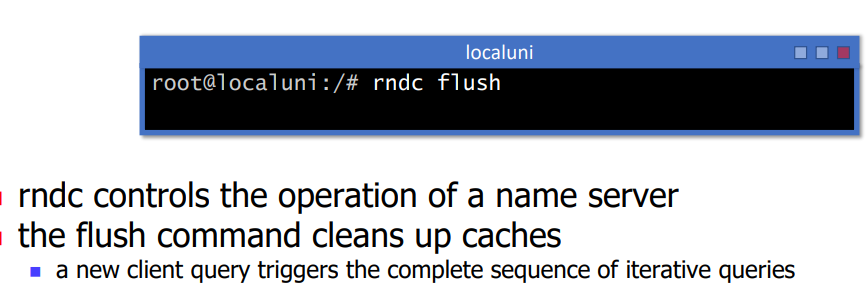
\includegraphics[width=16cm, height=3cm]{immagine_2025-01-04_131146854.png} % Percorso dell'immagine
    \caption{} % Didascalia per l'immagine
    \label{fig:immagine} % Etichetta per riferimento
\end{figure}
\noindent
Ora eseguiamo un esperimento mandando un ping verso un dispositivo inesistente, quello che succederà è che a causa della pulizia della cache tutte le query iterative verranno rifatte, fino a quando si accorgeranno che il dominio richiesto non esiste. Quando la query ritornerà failed \textbf{pc1} riprova una seconda volta con il percorso di ricerca del dominio configurato nel suo /etc/resolv.conf:\\
nameserver 192.168.0.11\\
search uniroma3.it\\
Se ripetiamo ancora una volta il ping verso un dispositivo inesistente, la negative cache del name server avrà memorizzato l'esito negativo quindi restituirà subito l'esito e pc1 riproverà con il percorso di ricerca del dominio configurato nel suo /etc/resolv.conf.
\subsection{Il comando dig}
I resource record possono essere cercati utilizzando il comando \textbf{dig}.
\begin{figure}[H] % Usa 'H' per forzare la posizione qui
    \centering % Centra l'immagine
    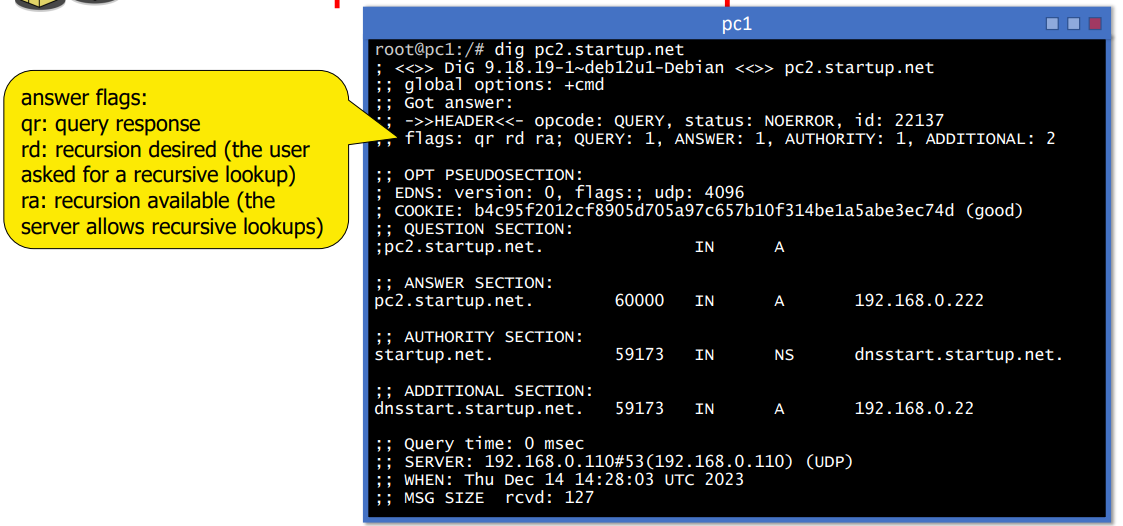
\includegraphics[width=17cm, height=8cm]{Screenshot 2025-01-04 131851.png} % Percorso dell'immagine
    \caption{} % Didascalia per l'immagine
    \label{fig:immagine} % Etichetta per riferimento
\end{figure}
\noindent
Le sezioni corrispondono a quelle contenute nei pacchetti DNS. Un messaggio DNS non caontiene mai più di una sezione di domanda. Nella sezione delle risposte invece potrebbero essere più di uno. Quei numeri ad es. (60 000) sono i TTL dei resource record e possono decrementare o rimanere costanti se il record è  memorizzato sul name server.
\begin{figure}[H] % Usa 'H' per forzare la posizione qui
    \centering % Centra l'immagine
    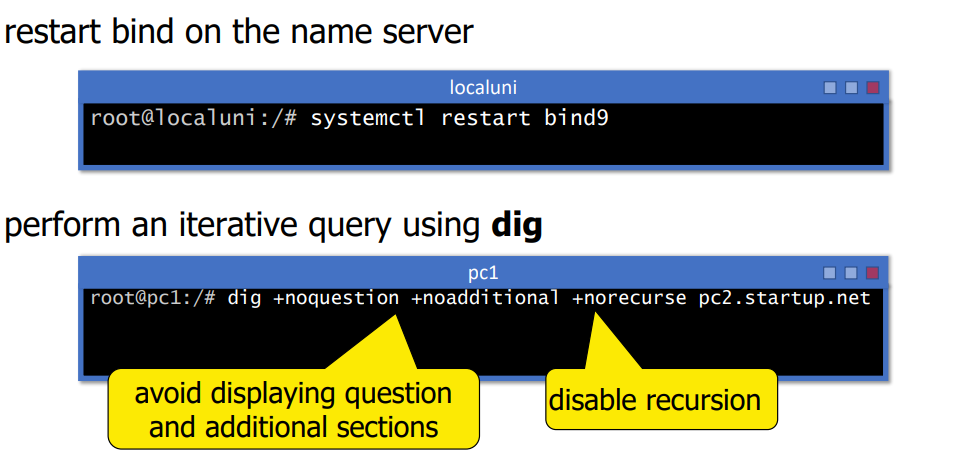
\includegraphics[width=17cm, height=6cm]{immagine_2025-01-04_132425944.png} % Percorso dell'immagine
    \caption{} % Didascalia per l'immagine
    \label{fig:immagine} % Etichetta per riferimento
\end{figure}
\noindent
Il server risponde specificando il name server autorevole da contattare per ottenere le informazioni desiderate. 
\begin{figure}[H] % Usa 'H' per forzare la posizione qui
    \centering % Centra l'immagine
    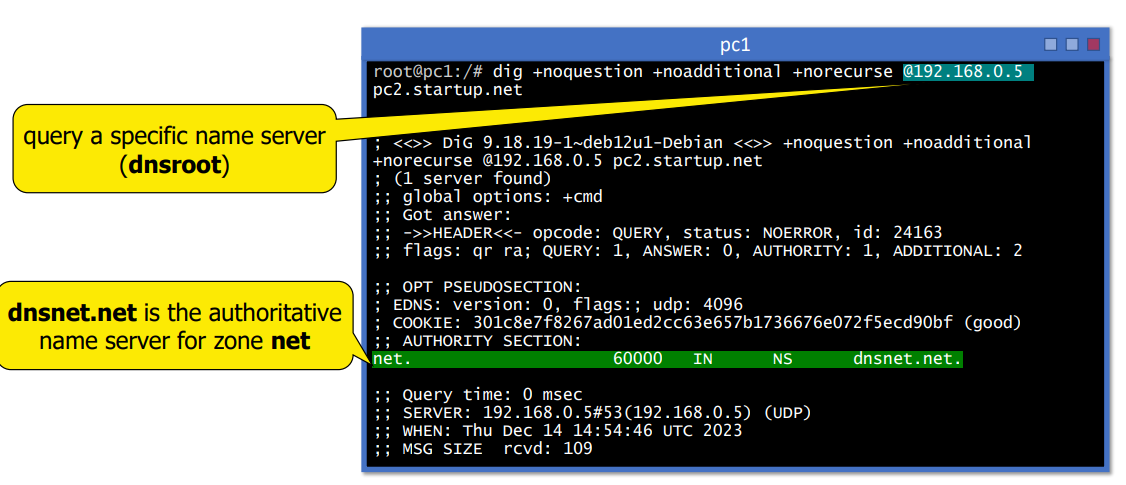
\includegraphics[width=17cm, height=6cm]{immagine_2025-01-04_132657207.png} % Percorso dell'immagine
    \caption{} % Didascalia per l'immagine
    \label{fig:immagine} % Etichetta per riferimento
\end{figure}
\noindent
Scendendo sempre di più con i name server arriveremo a \textbf{dnsstart.startup.net} il quale ci restituirà come riposta l'indirizzo di \textbf{pc2.startup.net}
\section{Sesto Lab: web server e browser}
\begin{figure}[H] % Usa 'H' per forzare la posizione qui
    \centering % Centra l'immagine
    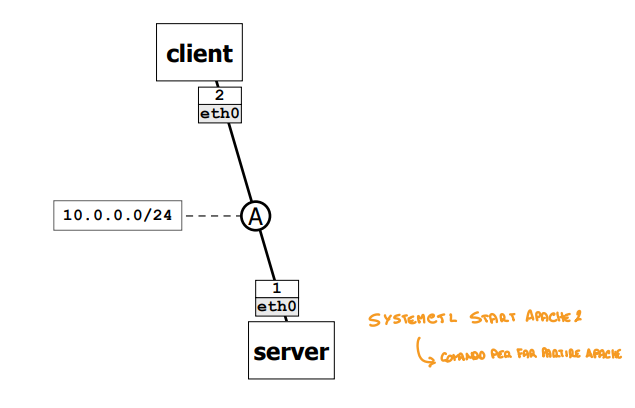
\includegraphics[width=11cm, height=5cm]{immagine_2025-01-06_142606968.png} % Percorso dell'immagine
    \caption{} % Didascalia per l'immagine
    \label{fig:immagine} % Etichetta per riferimento
\end{figure}
\noindent
Il server esegue \textbf{apache2}. Il client utilizza un web browser text-based (\textbf{links}) per controllare le operazioni del server.
\textbf{systemctl start apache2} per eseguire apache. Successivamente il client esegue \textbf{links http://10.0.0.1} per inizializzare il web browser. Successivamente attacchiamo \textbf{wireshark} per vedere cosa succede. Catturiamo 13 pacchetti che sono gli stessi che avevamo visto per HTTP.
\begin{figure}[H] % Usa 'H' per forzare la posizione qui
    \centering % Centra l'immagine
    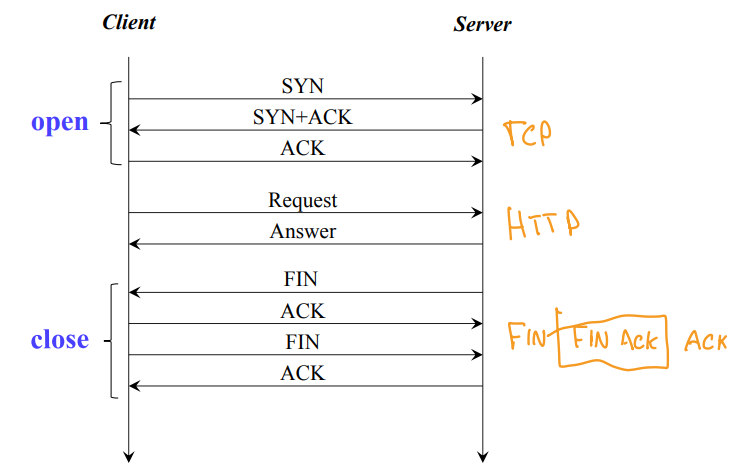
\includegraphics[width=11cm, height=4cm]{immagine_2025-01-06_143211571.png} % Percorso dell'immagine
    \caption{} % Didascalia per l'immagine
    \label{fig:immagine} % Etichetta per riferimento
\end{figure}
\noindent
(Apri wireshark per seguire meglio)\\
Il primo pacchetto è un \textbf{ARP Request} il client cerca il MAC address del server. Il secondo è un \textbf{ARP Reply} il server gli fornisce l'indirizzo MAC. Ora inizia il \textbf{three-way-handshake}. Nel primo pacchetto il client propone il sequence number e una grandezza massima del segmento (1460byte). Il secondo pacchetto è un \textbf{syn ack} in cui si conferma la grandezza massima del segmento, ora il server propone il suo sequence number iniziale e conferma quello proposto dal client. L'ultimo pacchetto è un \textbf{ACK} in cui il client conferma il sequence number proposto dal server. Il sesto pacchetto è un pacchetto \textbf{HTTP GET} a cui segue il settimo pacchetto in cui viene confermato il GET da \textbf{TCP}. Nell'ottavo pacchetto c'è la \textbf{risorsa richiesta}. Nel nono \textbf{TCP} conferma con un \textbf{ACK} la risorsa. Dopo il decimo, finisce la conversazione e quindi \textbf{FIN, ACK, FIN, ACK}.
\end{document}
